%\newpage
\section{Admixture from other channels}
\mbox{}\vspace{-\baselineskip}



%\afterpage{\clearpage}
Let's assume that some events in the sample correspond to the background channel with a greater number of final state particles, i.e. $ep\rightarrow e'p'\pi^{+}\pi^{-}x$. Then, for such background events, the following relations for the missing quantities can be obtained,
\begin{equation}
\begin{aligned}
&M_{X[0]}^{2}&=&~\left [P_{X[0]}^{\mu} \right ]^{2}&=&~[P^{\mu}_{x}]^{2} = m_{x}^{2} >0~~\textrm{and}\\
&M_{X[\pi^{-}]}^{2}&=&\left [P_{X[\pi^{-}]}^{\mu}\right ]^{2}&=&~(P_{\pi^{-}}^{\mu}+P^{\mu}_{x})^{2}=[P^{\mu}_{\pi^{-}}]^{2} +[P^{\mu}_{x}]^{2}+2\left [P_{\pi^{-}}\right ]_{\mu} P_{x}^{\mu} \\
&&&&=&~m_{\pi^{-}}^{2} + m_{x}^{2} +2(E_{\pi^{-}}E_{x} - (\overrightarrow{p}_{\pi^{-}}\cdot \overrightarrow{p}_{x}))  \\
&&&&>&~m_{\pi^{-}}^{2} + m_{x}^{2}+2m_{\pi^{-}}m_{x} > m_{\pi^{-}}^{2},\\
\end{aligned}\label{eq:mm_other_ch}
\end{equation}
where $P^{\mu}_{x}$ is the four-momentum of the extra particle $x$ and $m_{x}$ is its mass.




Thus, in the distribution of the quantity $M_{X[0]}^{2}$, the background events form an additional discrete narrow peak located on the right side of the main peak at the position of $m_{x}^{2}$. Meanwhile, the background in the distribution of $M_{X[\pi^{-}]}^{2}$, being also well-separated from the main peak and located on its right side, forms a broad structure, which starts at the value of $m_{\pi^{-}}^{2} + m_{x}^{2}+2m_{\pi^{-}}m_{x}$.



This situation is illustrated in Fig.~\ref{fig:mm_backgr} for the case when the extra particle is $\pi^{0}$. The plots are produced by means of the GENEV event generator~\cite{Genev}.



\begin{figure}[htp]
\begin{center}
\framebox{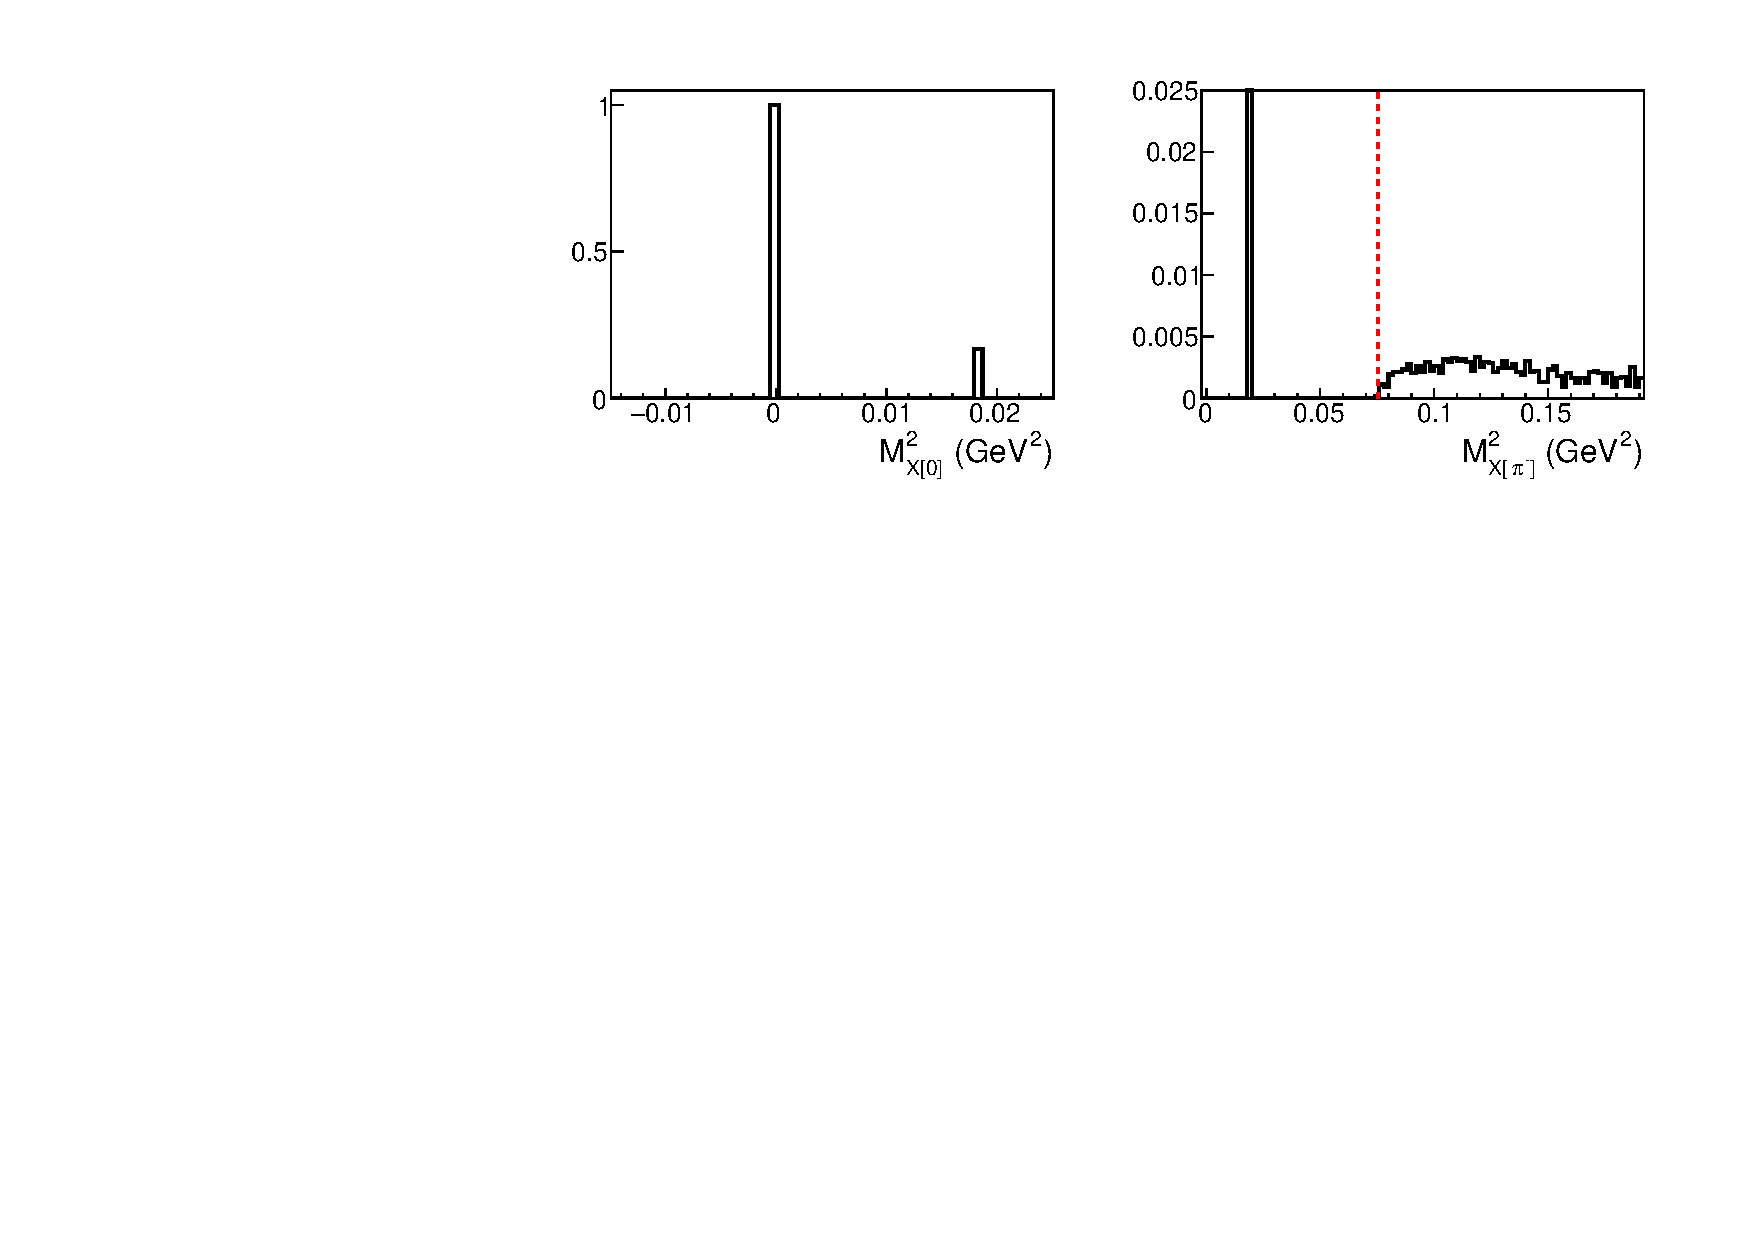
\includegraphics[width=\textwidth]{pictures/mm_other_ch2.pdf}}
\caption{\small Distributions of the quantities $M_{X[0]}^{2}$ (left) and $M_{X[\pi^{-}]}^{2}$ (right) plotted for the event sample that contains the background admixture from the channel $ep\rightarrow e'p'\pi^{+}\pi^{-}\pi^{0}$. The discrete right peak (left panel) and the right-side structure (right panel), both well-separated from the main peak, are formed by the background events. The right plot is zoomed in on small $y$, and the red dashed line there marks the value of $m_{\pi^{-}}^{2} + m_{\pi^{0}}^{2}+2m_{\pi^{-}}m_{\pi^{0}}$.   } \label{fig:mm_backgr}
\end{center}
\end{figure}


